\documentclass[conference]{IEEEtran}
\usepackage[utf8]{inputenc}
\usepackage{amsmath}
\usepackage{changepage}
\usepackage{graphicx}
\usepackage{float}
\usepackage{amssymb}
\usepackage{array}
\usepackage[english]{babel}
\usepackage{authblk}
\title{Open Source Software Framework for Indoor Geolocation Using 802.11 Protocol}

\date{April 2018}
\usepackage[backend=bibtex,style=numeric,sorting=none]{biblatex}
\bibliography{main.bib} 
\begin{document}
\author[1]{Paul Bryden\thanks{Paul.Bryden.2014@uni.strath.ac.uk}}
\author[2]{Kinjal Gala\thanks{kgala@sdsu.edu}}
\author[2]{Christopher Paolini\thanks{cpaolini@sdsu.edu}}
\author[2]{Mahasweta Sarkar\thanks{msarkar@sdsu.edu}}
\affil[1]{Department of Electronic and Electrical Engineering, University of Strathclyde}
\affil[2]{Department of Electrical and Computer Engineering, San Diego State University}

\renewcommand\Authands{ and }
\maketitle
\begin{abstract}
One in Four Americans over the age of 65 falls every year [1].  Most of these falls are very serious and can result in major mobility injuries and/or death. The shorter the amount of time it takes for fall victims to get medical attention, the greater their odds of recovery. As such, it would be very beneficial to develop an Open Source Software Framework capable of identifying the location of a victim within a building, or indoor environment, using existing infrastructure. 
\newline \indent This paper discusses the development of a platform-agnostic open source software framework capable of deriving the location of an individual down to 3m accuracy using 802.11 WiFi protocol (in areas of good WiFi coverage). A complete end to end framework has been sketched and is comprised of the sensor software (embedded layer), Web Services and a mobile application for monitoring the movements of individuals. The location of a user is calculated using trilateration and Kalman Filtering is employed to reduce the effect of multipath interference. The software framework is written mostly in C++11 and takes full advantage of modern Object Oriented design principles to ensure platform portability and flexibility. The solution provides a real, no cost, an extendible solution to the problem of indoor geolocation and it is hoped that many individuals will benefit from this work.
\end{abstract}
\section{Introduction}
\indent According to the Centers for Medicare and Medicaid Services (CMS), health-care in the United States has seen a tremendous growth in the past decade. The CMS projects a 5.9\% growth increase in 2018 and projects national health spending to be 19.9\% of GDP. The maximum percentage of funds allocated to health care is needed by people above the age of 55, which comprises approximately 29\% of the American population \cite{hi}. The primary reasons for injuries in elderly people are falls due to their debility with respect to their age. Some of these injuries can be fatal or may create a psychology of fear in the individual, resulting in them losing the ability to walk properly after a fall. Many algorithms and embedded technologies have been in research and development for the past several years, which aim to work towards the basic goal of detecting a fall and reporting the location of the fallen individual to a respective authority.
\newline  Indoor geolocation tracking is an evolving technology which aims the derive the location of an individual within an indoor environment. One of the promising classes of this emerging technology is to take advantage of existing infrastructure to determine the location of a user. \cite{pahlavan2002indoor}. Much work has been carried out to use GPS for indoor location tracking \cite{kjaergaard2010indoor}. However, GPS has an only has an accuracy of 5-50m in an indoor environment. \cite{liu2007survey}.
\newline \indent This paper presents the development of an open source software platform capable of tracking the movements of individuals using existing 802.11 WiFi Infrastructure. The modularity of the Software Framework developed, and its strong use of C++11 design principles, also enables it to be easily adapted to a variety of hardware platforms and radio technologies such as Bluetooth or LoraWAN.
\section{Background}
\noindent  The ability to identify the geographic location of an individual residing outside of a building by latitude, longitude, and altitude is easily accomplished using a relatively inexpensive GPS receiver. Typical commercially available receivers for under \$100 can provide coordinates within a sampling time of 30s to an accuracy of \newcommand{\rpm}{\raisebox{.2ex}{$\scriptstyle\pm$}} 3m. For example, the Copernicus II 12-channel GPS module from Trimble is under \$70 and can provide updated coordinates with a period of 3s. GPS receivers typically use a carrier wave in the L1 band at 1575.42 MHz on which navigation messages are modulated. Unfortunately, such microwave signals are significantly attenuated by building roofs and walls, rendering GPS unusable indoors [2].
Indoor position measurements can be accomplished using different mechanisms such as radio signals, magnetic fields, and sound waves. Newer, emerging technologies employ computer vision to identify objects in the field of a camera's view. The vision system can then measure distances in between recognized objects, and between the user and recognized objects. These measurements provide a system with depth perception and can identify how far a user is away from a surface or other rigid body in a field of view.
This research project utilizes radio signals, specifically radio signals from 802.11 WiFi access points. After calculating the known location of these access points and the signal strength at a receiver, the distance can be derived using a modification of the free space equation. In this software framework, four access points are employed to derive the location of the user by calculating the distance between them using trilateration.
\section{Software Framework Architecture}
The software framework, presented in this paper, is composed of three components.
\newline
1) Embedded Layer
\newline
2) Middleware Layer
\newline
3) Mobile Application Layer
\newline
The embedded layer is comprised of all of the software which runs on the sensor node held by the user.
The middleware layer is comprised of RESTful Web Services and a PostgreSQL database, which connects the Embedded and Mobile Application layers.
The mobile application layer consists of an Android Application, which is used to render a user's location.
A diagram of the complete software framework is shown in Figure 1.
\begin{figure}[H]
    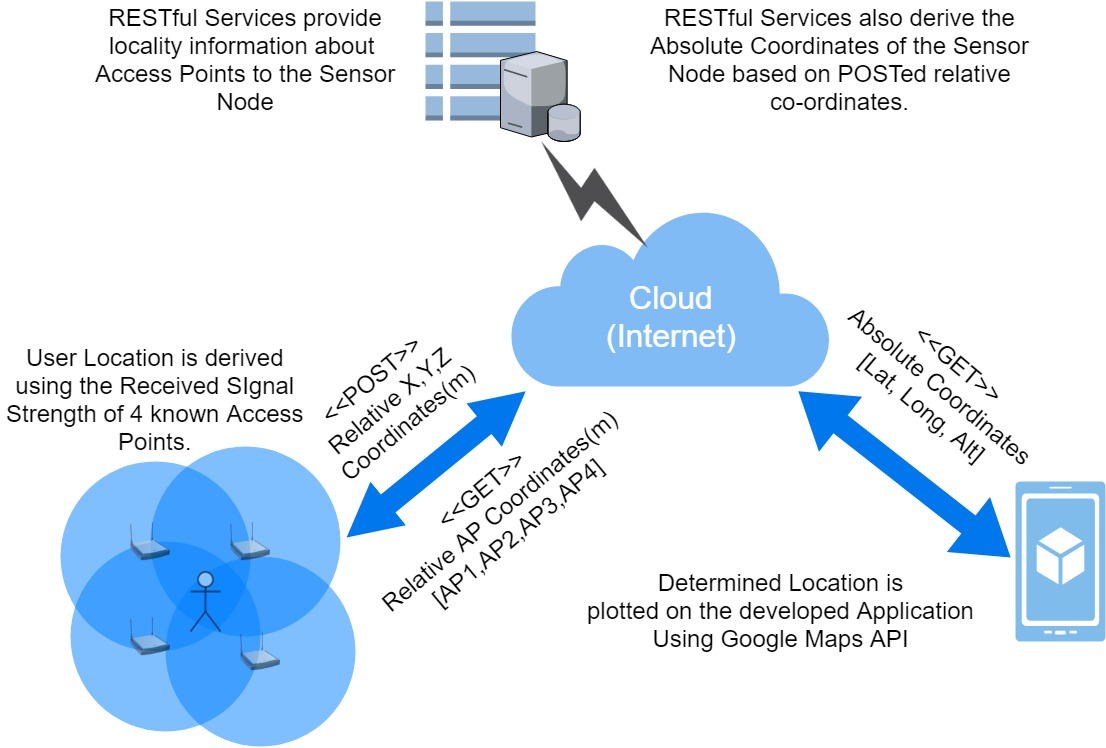
\includegraphics[width=9 cm,height=5.5 cm]{System_Diagram.jpg}
    \caption{Software Framework Architecture Overview}
    \end{figure}
The RESTful API is the fundamental interface between all components of the software framework. In terms of data flow, the Web Services provide the relative coordinates of known access points to the sensor node, and the node responds with the relative X, Y, Z coordinates (m) of its own derived location. The Web Services then translate these coordinates into absolute latitude, longitude, and altitude which are consumed by a mobile application.
The 3 respective layers and their operation will now be discussed in detail.
\subsection{Embedded Layer}
The embedded layer is the component of the software framework which runs on a sensory device operated or worn by a user. The embedded layer was written in C++ using design principles and is portable across Linux, Windows, iOS, Android, and other platforms. This portability is possible thanks to the use of modern OOP design principles and the employment of cross-platform libraries as BOOST and CPPRestSDK, which removes platform awareness for the majority of the system. As one can see from Figure 2, the only part of the system that requires awareness of the underlying OS/Platform is the Node Scanner Module. A Node in the framework is defined as an 802.11 Access Point. Direct OS interaction is required at this layer due to the low level of access required to the wireless hardware.
BOOST is used mainly to enable straightforward, cross-platform, thread safety and thread handling and the CPPRestSDK are used to handle JSON construction and parsing along with HTTP Requests.
\begin{figure}[H]
    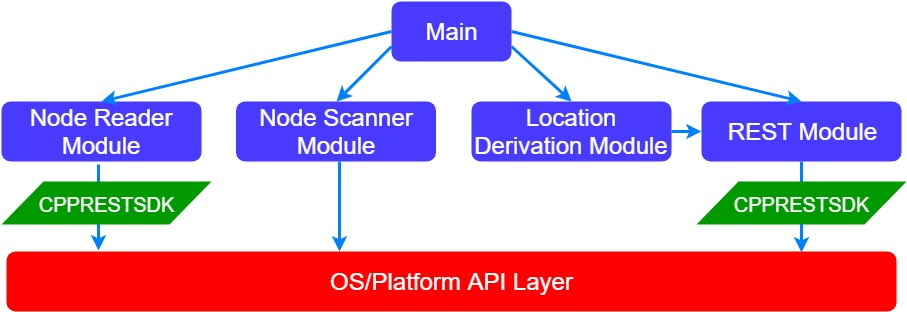
\includegraphics[width=9 cm,height=3.5 cm]{Pink_Panther_Architecture.jpg}
    \caption{Embedded Layer Architecture}
    \end{figure}

\subsubsection{Modules Overview}
\rule[-10pt]{0pt}{10pt}\\
 Node Reader Module:
\newline
The Node Reader Module is responsible for creating a known list of nodes and their locations.  This has been implemented in two different flavors - a file reader, and a HTTP GET reader. The recommended module to utilize is the HTTP GET reader. This module simply grabs the known list of nodes in JSON format from the middleware Web Services and populates a list of nodes known to the Location and REST Modules.
\newline
\newline
Node Scanner Module:
\newline
The Node Scanner Module is responsible for interfacing with the OS or Platform API which provides the data from a WiFi Scan - or other radio platform. It provides a list of Nodes populated with RSSI (Received Signal Strength).
\newline
\newline
Location Derivation Module:
\newline
The Location Derivation Module is responsible for deriving the exact X,Y and Z co-ordinates of the user node, based on the data from the Node Reader and Node Scanner Modules. The details of the implementation will be discussed in the theory of trilateration and implementation sections.
\newline
\newline
REST Module:
\newline
The REST Module is responsible for posting the data from the Location Derivation Module to the Web Services. It is also responsible for providing the data to any interested party through a GET route.
\newline
\subsubsection{Theory of Trilateration}
In order to derive the relative location of a particular sensor node, trilateration techniques will be employed. The theory of the particular techniques employed will be discussed and the effectiveness of the solution documented. Fundamentally, the ability to derive the location of the sensor node comes from the ability to measure  the  Received  Signal  Strength (RSS) of  several  different  WiFi  access  points (APs)  within  32m  of  the  user.    Typically,  the  received  signal  power  within  one  meter  of  an  AP  will  be  approximately  -32  dBm,  and  close  to  -90  dBm  at  a  distance  of  32m. The RSS can be  modeled using  equation  (1)  
\begin{equation}
RSS = 10N*\log_{10}D-A  
\end{equation}
where: 
\newline
N = Signal propagation constant
\newline
A = Received signal strength at 1 meter (dBm)
\newline
D = Distance in (m)
\newline
\newline
The optimal signal propagation constant for a noisy indoor environment was found to be approximately 2.5. With  4 or more  Access Points,  one  can  use  trilateration  to  locate  a  user  using  four  distances  computed  from  four  RSS  values.    Let  ( x , y , z )  represent  the  unknown  location  of  a  user  and $(d_1,  d_2,  d_3,  d_4)$ represent 4 distance values obtained from the measured RSS between user's Embedded Wireless Device and Four Access Points. The System of Euclidian  distances  between  the  user  and  four  Access Points  is  given  by  equations below:

\begin{equation}
x-x_1^2 + y-y_1^2 + z-z_1^2 =d_1^2
\end{equation}
\begin{equation}
 x-x_2^2 + y-y_2^2 + z-z_2^2 =d_2^2 
\end{equation}
\begin{equation}
 x-x_3^2 + y-y_3^2 + z-z_3^2 =d_3^2 
\end{equation}
\begin{equation}
 x-x_4^2 + y-y_4^2 + z-z_4^2=d_4^2 
 \end{equation}
 \newline Subtracting rows 2, 3 and 4 from row 1, the following set of equations can be derived.
\begin{equation}
\resizebox{0.9\hsize}{!}{$2(x_2 - x_1) + 2(y_2 - y_1)y + 2 (z_2 - z_1)z = x_2^2 - x_1^2  + y_2^2 - y_1^2 + z_2^2 - z_1^2 - d_2^2 +d_1^2$}
\end{equation}
\begin{equation}
\resizebox{0.9\hsize}{!}{$2(x_3 - x_1) + 2(y_3 - y_1)y + 2 (z_3 - z_1)z = x_3^2 - x_1^2 + y_3^2 - y_1^2 + z_3^2 - z_1^2 - d_3^2 +d_1^2$}
\end{equation}
\begin{equation}
\resizebox{0.9\hsize}{!}{$2(x_4 - x_1) + 2(y_4 - y_1)y + 2 (z_4 - z_1)z = x_4^2 - x_1^2 + y_4^2 - y_4^2 + z_4^2 - z_1^2 - d_4^2 +d_1^2$}
\end{equation}
The System can be expressed in Ax=b matrix form as
 \newline
 \\* 
 
\begin{equation}
\resizebox{0.9\hsize}{!}{
$\left[ \begin{array}{ccc}
(x_2 - x_1) & (y_2 - y_1) & (z_2 - z_1)\\
(x_3 - x_1) & (y_3 - y_1) & (z_3 - z_1) \\
(x_4 - x_1) & (y_4 - y_1) & (z_4 - z_1) \\
\end{array} \right] 
% 
\left[ \begin{array}{c}
x \\
y\\
z\\
\end{array} \right]
%
= 1/2 
\left[ \begin{array}{c}
x_2^2 - x_1^2 + y_2^2 - y_1^2 + z_2^2 - z_1^2 - d_2^2 + d_1^2 \\
x_3^2 - x_1^2 + y_3^2 - y_1^2 + z_3^2 - z_1^2 - d_3^2 + d_1^2 \\
x_4^2 - x_1^2 + y_4^2 - y_1^2 + z_4^2 - z_1^2 - d_4^2 + d_1^2 \\
\end{array} \right]
$}
\end{equation}
\\*
\newline and solved using a Gauss - Newton least squares approximation. 
\begin{equation}
(A^TA)X = A^Tb
\end{equation}
\newline
Since A is constant, the system of equations can also be solved by simply using back substitution or least uppers squares estimate.
\newline
However, multipath  effects,  co-channel  interference  (CCI), and  adjacent-channel  interference can  affect  the  SNR,  resulting  in  location  measurement  error. In an attempt to mediate the error introduced by such environmental effects, Kalman Filtering will be employed.
\newline
\subsubsection{Theory of Extended Kalman Filter}
RSS (Received Signal Strength) value depends directly, and only, on the distance between the 802.11 WiFi transmitter and the receiver – in an ideal system. In reality, however, multipath interference, Electromagnetic interference and signal fading all play a significant role in causing fluctuations in the Received Signal Strength. As such, it is required that the RSS values are filtered in the time domain such as to mitigate the effect of such noise. One such method is through the use of an extended Kalman Filter. The equations representing the implemented Kalman filter can be seen below and are executed on each "tick" of the system \cite{KalmanFilter}.
\begin{equation}
p = p + q
\end{equation}
\begin{equation}
k = p / (p + r)
\end{equation}
\begin{equation}
x = x + k * (i - x)
\end{equation}
\begin{equation}
p = (1 - k) * p
\end{equation}
where:
\newline
q is the Process Noise Covariance \\
r  is the Measurement Noise Covariance \\
x is the Kalman Filtered Value \\
p is the Estimation Error Covariance \\
k is the Kalman Gain \\
i is the most recently measured RSSI value\\

\noindent Measurement Covariance is the standard deviation of a set of measured results – determined to be 2.36dBm This was derived by taking several measurements of the RSSI (dBm) at a 1m distance from an 802.11 Wireless Access Point in the test environment. The Process Covariance is the susceptibility of the system to change - determined to be 0.001. This was determined through trials to best match the typical speed at which an individual may move around a facility.
\newline
\subsubsection{Implementation}
The Embedded Layer was implemented in a very modular fashion using OOP and C++11 design principles. These include but are not limited to polymorphism, inheritance, decorator and singleton patterns. Such modern C++ features as shared pointers, scoped locks, tasks and initializer lists were also heavily utilized.
The employment of these principles and features has enabled a very flexible, thread-safe, memory safe system to be constructed and portable across multiple platforms. The UML for the completed system can be seen in Figure 3.

\begin{figure}[H]
    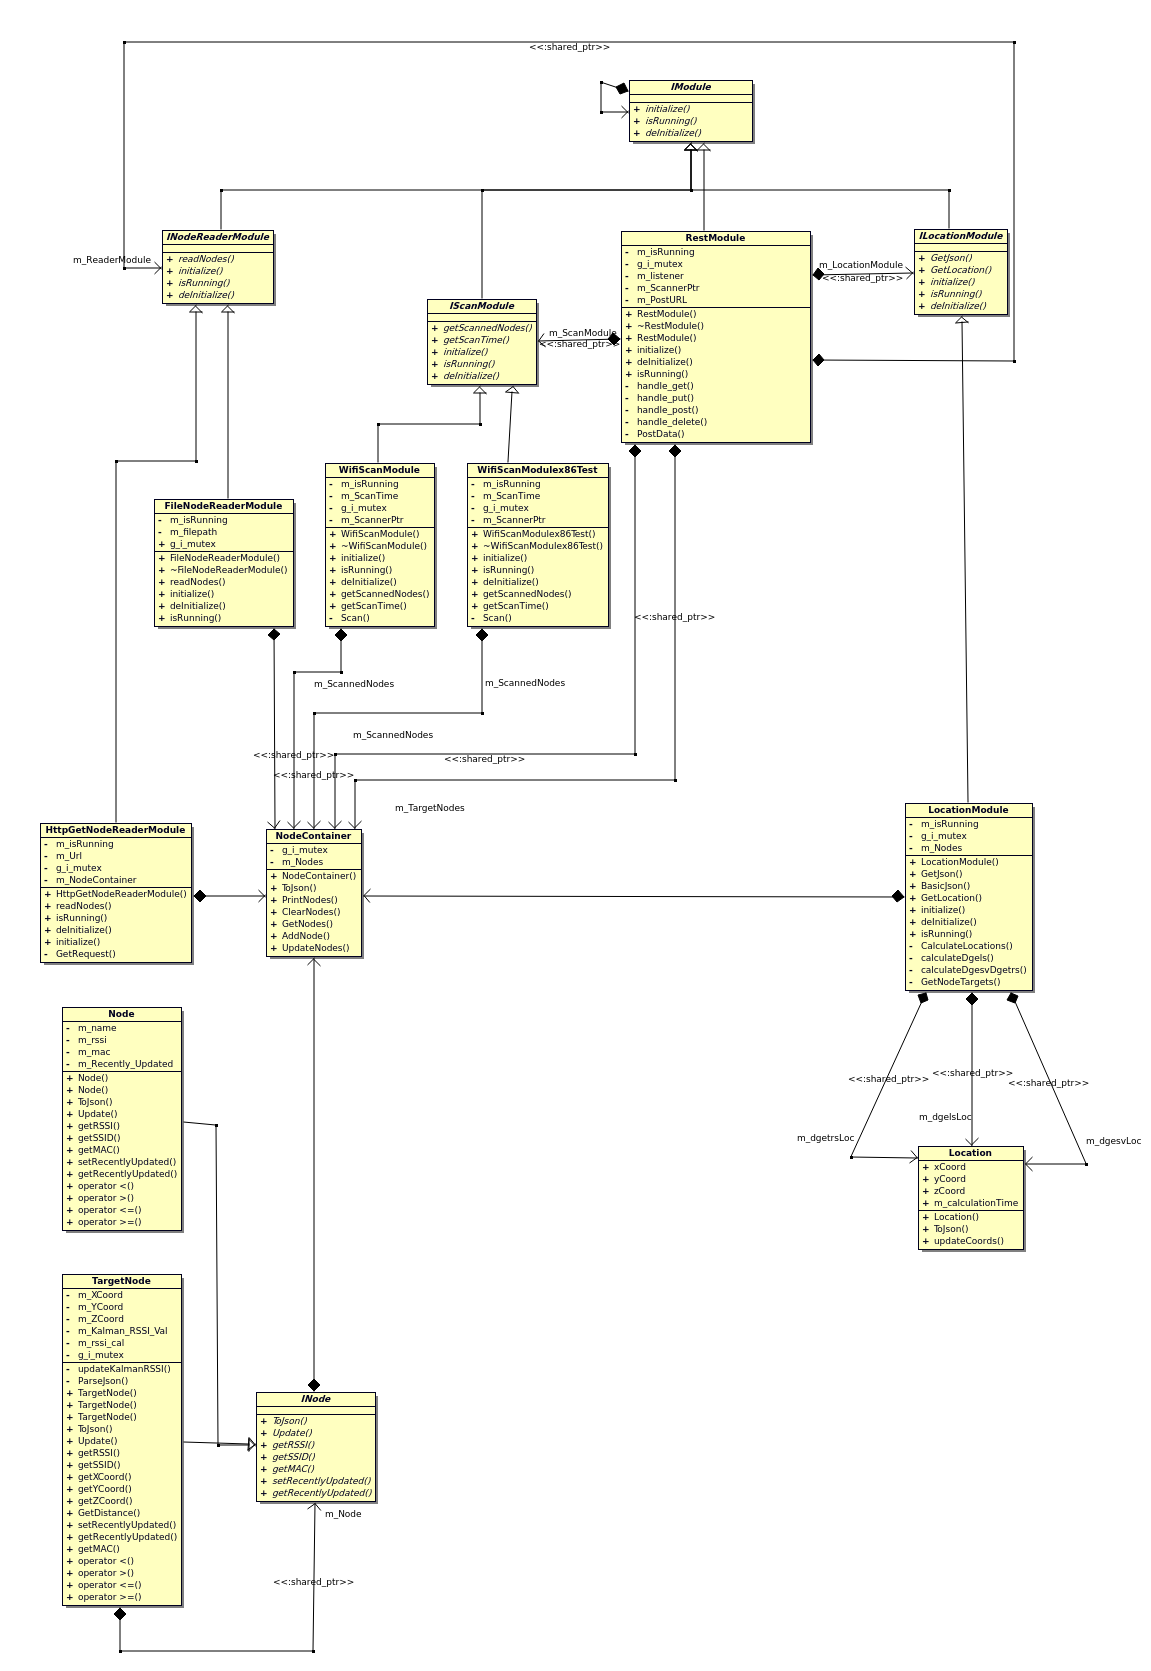
\includegraphics[width=9cm,height= 9 cm]{uml_9-5-18.png}
    \caption{UML Diagram of Embedded Layer}
    \end{figure}

The system comprises 2 core components:
\newline
Module Classes: These are the core drivers of the system. Each module provides the system with discrete functionality. Some modules, such as the Rest Module, rely on other modules to enable operation, however, they do not depend on a particular implementation of those modules. \newline
There are 4 key modules which make up this system:
\newline
The Location Module Class - This module is responsible for deriving the exact location of the user based on the 4 nodes with the best signal strength in the target node container. In this open source framework, the LAPACK mathematical library is used to solve the systems of equations. 3 different methodologies for location derivation are employed; DGESV and DGELS for least squares approximation and DGETRS for back substitution.
\newline
The Rest Module Class - This module is responsible for providing the location, scan and target node list data to any interested parties by hosting the JSON on a GET Route. The module is also responsible for POSTing the derived location data to the remote Web Services server.
\newline
The Scan Module Class - This module is responsible for populating a list of nodes with the RSSI evident at the Beaglebone for each Access Point. This list can then be used to update the target nodes.
\newline
The Node Reader Module Class - This module is responsible for populating a list of "Target" Nodes. That is nodes which are of known location. This list can be obtained from a file in JSON format, using the file reader variant or from a web address using the GETreader variant.
\newline
 
Data Classes: These are the classes which all modules use to some extent. The "Data" classes are the Node, Node Container and Location Classes which store information relating to AP information or User location information. Node class objects are used to identify any node picked up in a scan. Target Nodes correspond to nodes of which the location is known and as such can be used for triangulation. Each target node is responsible for updating it's Kalman filtered location when a new RSSI value is provided. The location data class simply contains the X, Y and Z coordinates for a location and helper methods for accessing and modifying this data. 
\newline
The system is driven by the main class, where all of the modules are created and initialized. The main loop ensures the system is continuously scanning and updating the location as quickly as possible. A target node container is created and shared between the location module, node reader module and Scan Module. When the modules are initialized, the Node Reader Module updates that container with a list of target nodes, of known location, which is updated with RSSI measurements as is necessary through the Scan Module. The Location Module then employs this information to derive relevant, up to date location information. This information is then POSTed by the REST Module to the relevant web server and is also provided to anyone listener through a GET route.

\subsection{Middleware}
The Middleware comprises of 2 main components:\newline
The RESTful Web Services and the Back-end database. The Restful Web Services provide the API which both the Mobile Application and the Embedded Layer interact with. The Back End Database is where all location data related to known Access Points and User location is contained/amended. It is only interfaced with through the RESTful Web Services.
\newline
\subsubsection{RESTful Web Services}
The RESTful (Representational State Transfer) style Web Services were built using the JAVA Glassfish library and framework. These services  provide an interface to the data contained within the database - as well as a way to write derived location data to the database. 2 GET Routes were provided:\newline
1) A route which lists the known access points for a location in JSON format \newline
2) A route which lists the user's exact location (longitude, latitude, and altitude).
\newline
There is also 1 HTTP POST route which takes in x, y, z co-ordinates and a site number (in JSON format) derived by the embedded layer and writes the corresponding Latitude, Longitude, and Altitude into the PostgreSQL database.
\newline
\subsubsection{Back end Database}
PostgreSQL is the back end database where all the values that are pulled by the web-services including the exact location of the person are stored securely. The database consists of several tables including one pertaining information on known access point location and a moving window table containing last known location of the sensor nodes. In order to obtain the relative coordinates of each access point a common origin was placed in the southwest corner of each building, then the correct latitude and longitude of each access point were obtained by offsetting the latitude and longitude of the origin. Cartesian coordinates (m) of each AP relative to the corner of the building were stored in the database.
\newline

\section{Mobile Android Application}
 The Mobile Android Application was developed as a proof of concept to show the power of the developed system. The application simply GETs the relevant Long/Lat coordinates from the Web Services and renders them as a point using the Google Maps API. In addition, the architectural plans for the building being targeted are also rendered on the Google Map to enable individual rooms to be easily identified. The application was published on the App Store and it is possible for multiple individuals on different Android devices to utilize the application simultaneously. The application can be seen in Figure 4.
\begin{figure}[H]
    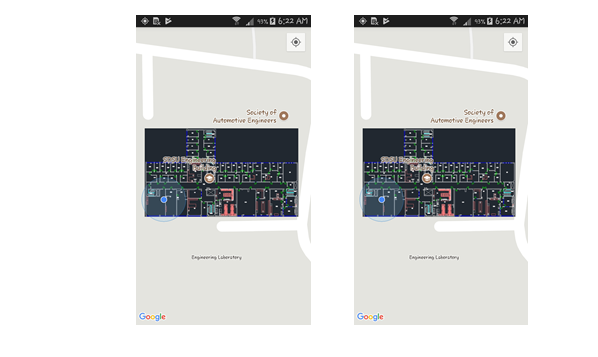
\includegraphics[width=8cm,height=5cm]{2018-05-10-PHOTO-00000078.png}
    \caption{Mobile Android Application Using Google Maps API}
    \end{figure}
\section{Testing and Results}
\subsection{Test Platform}
As one can see, a modular, flexible, portable, end to end, Open Source Framework has been developed, capable of deriving the location of a user using existing WiFi infrastructure. However, the accuracy of the system has not been discussed. In order to test the system, an embedded ARM Linux board called the Beaglebone was employed with a WiLink 8 chip. 2x 6dB, vertically polarized, high gain Antennae were employed to boost the RSSI (Received Signal Strength Indicator) present at the Wilink Chip. The solution was powered by a 2000mAh battery and was contained within a 3D printed housing. The solution can be seen in Figure 5.
\begin{figure}[H]
    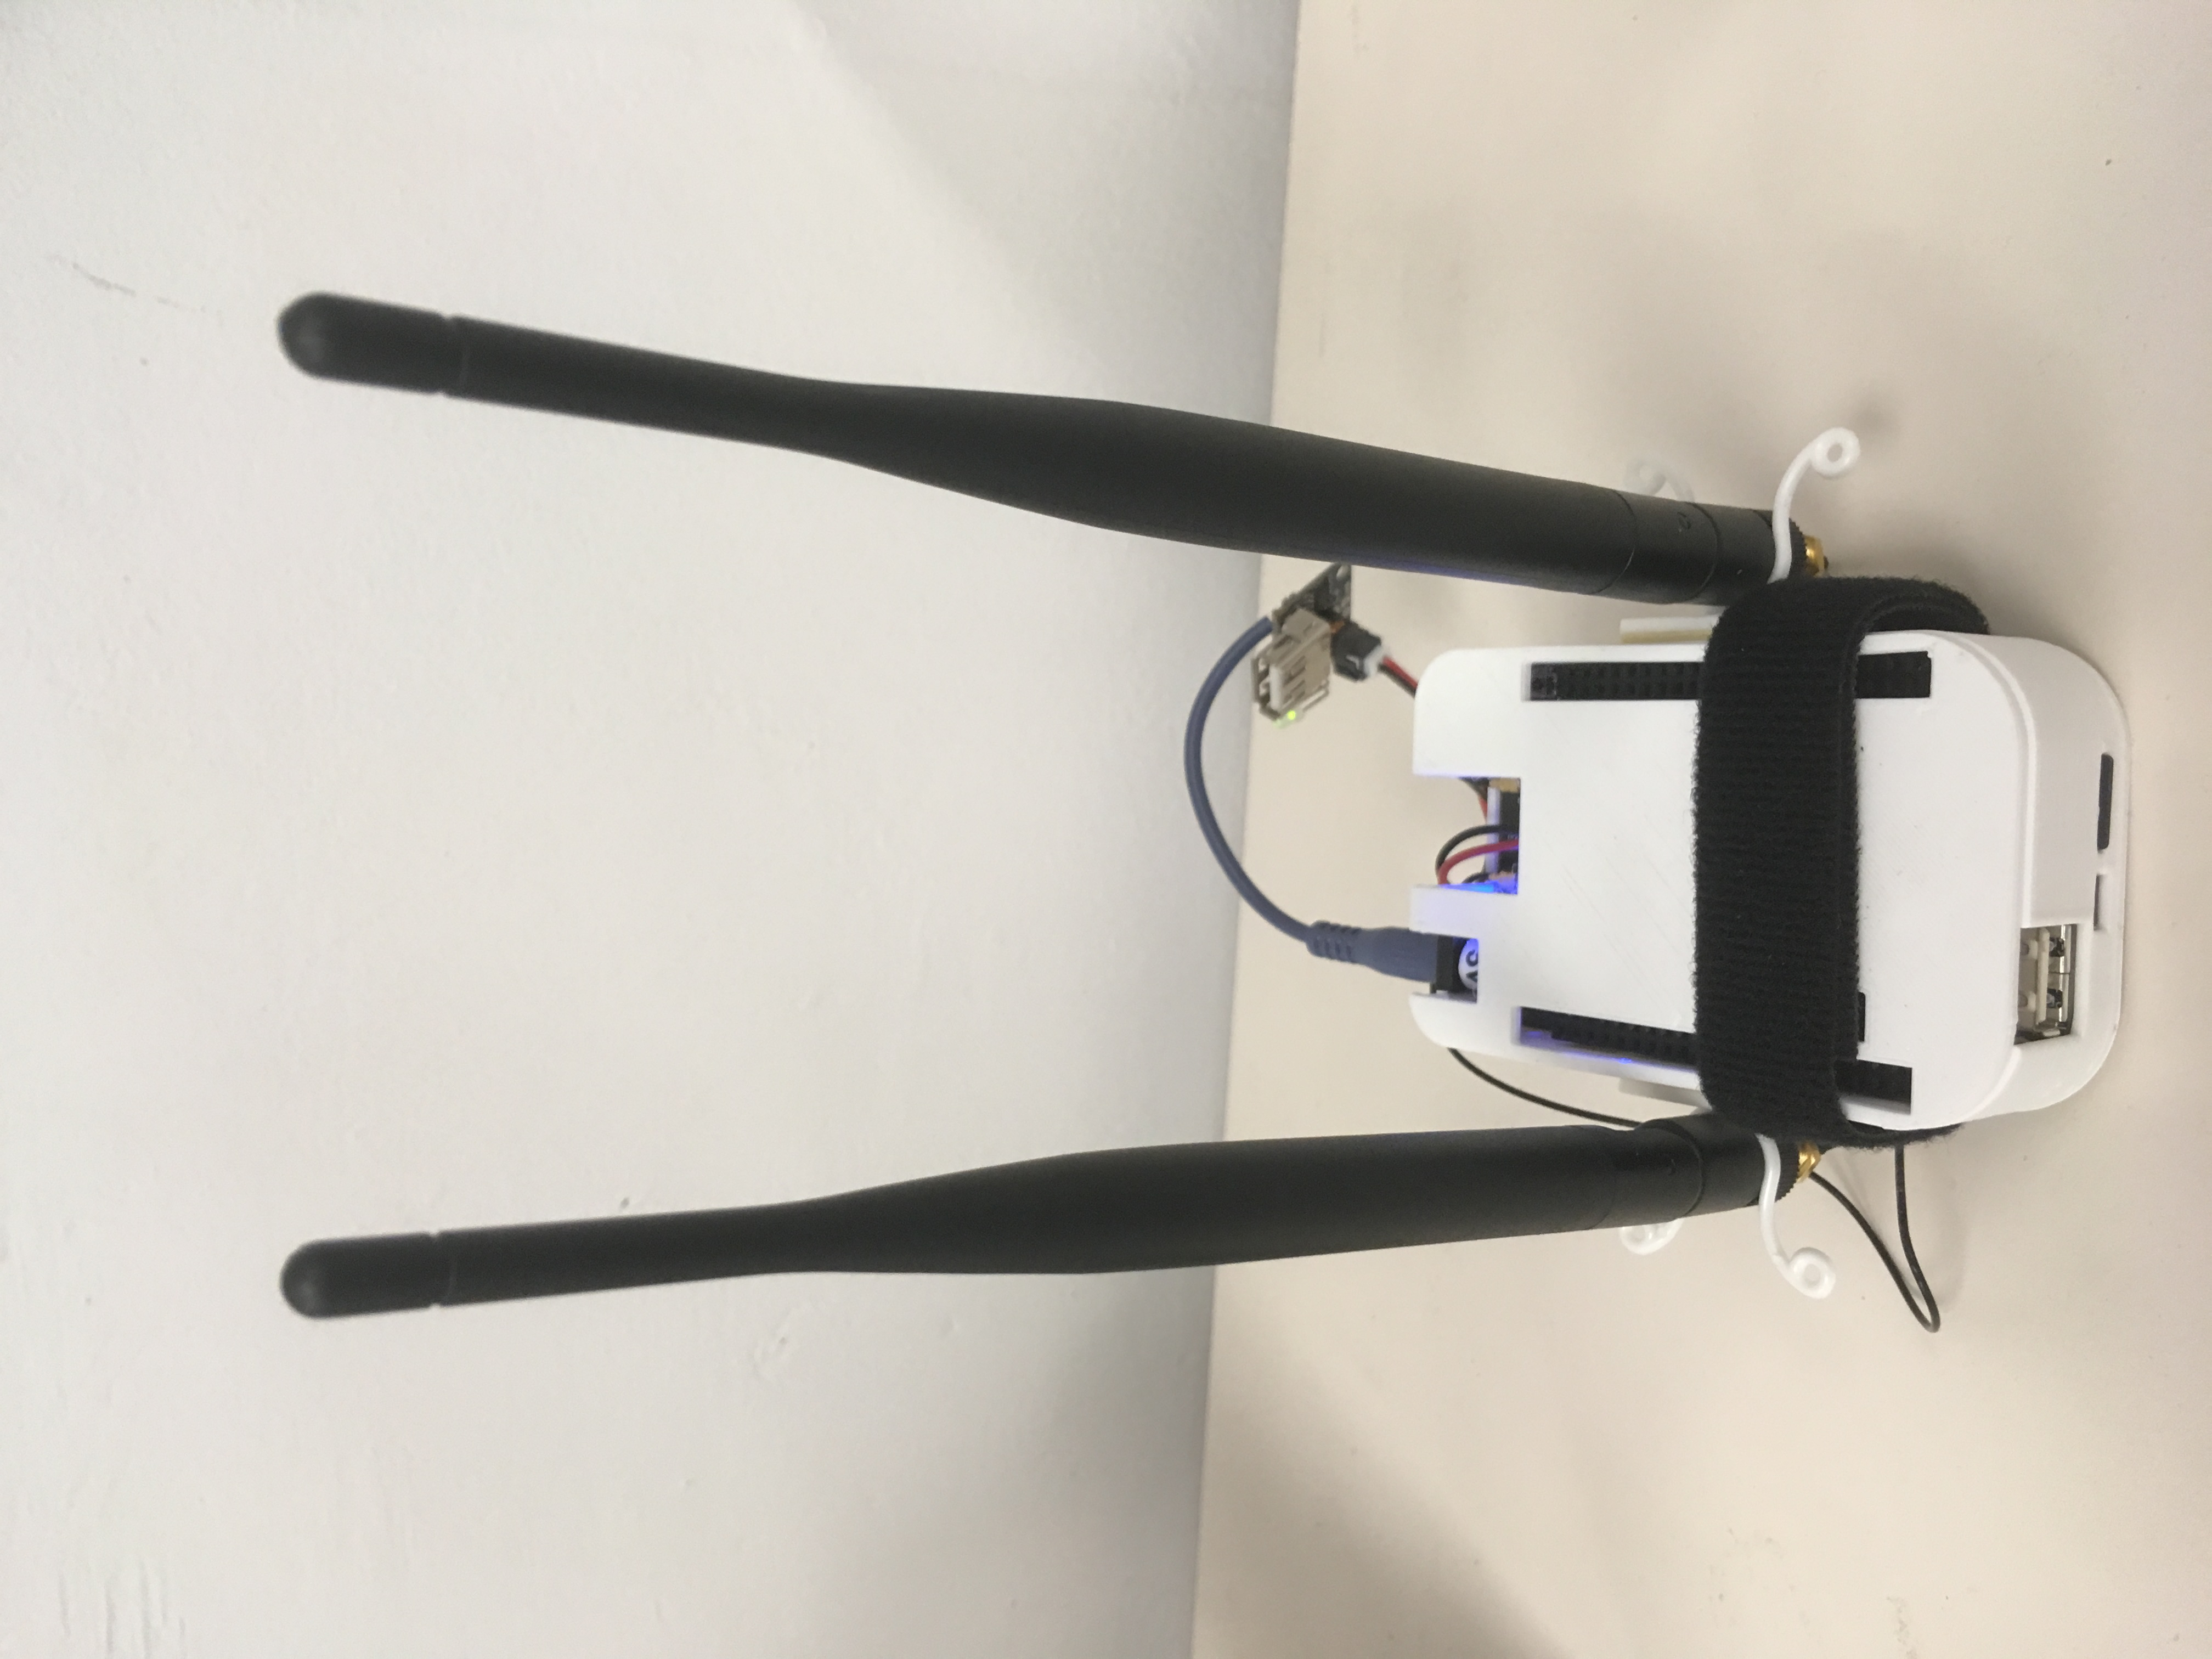
\includegraphics[width=8cm,height=5cm]{IMG_0796.JPG}
    \caption{Beaglebone Test Platform}
    \end{figure}

\subsection{Results}
In order to validate the effectiveness of the solution - multiple tests were completed to evaluate:\newline
i) The Kalman Filter \newline
ii) The execution time of the LAPACK functions\newline
iii) The effectiveness of the location complete derivation toolkit.

\subsubsection{Kalman Filter Results}
The Kalman Filter, and it's performance, was evaluated by stationing the test platform in a single location and comparing the raw RSSI data with the Kalman Filtered RSSI data. The location was a Wireless Technologies lab with high incidences of multipath interference and obstacle induced path loss. The results of the sampling can be seen in Figure 6.
\begin{figure}[H]
    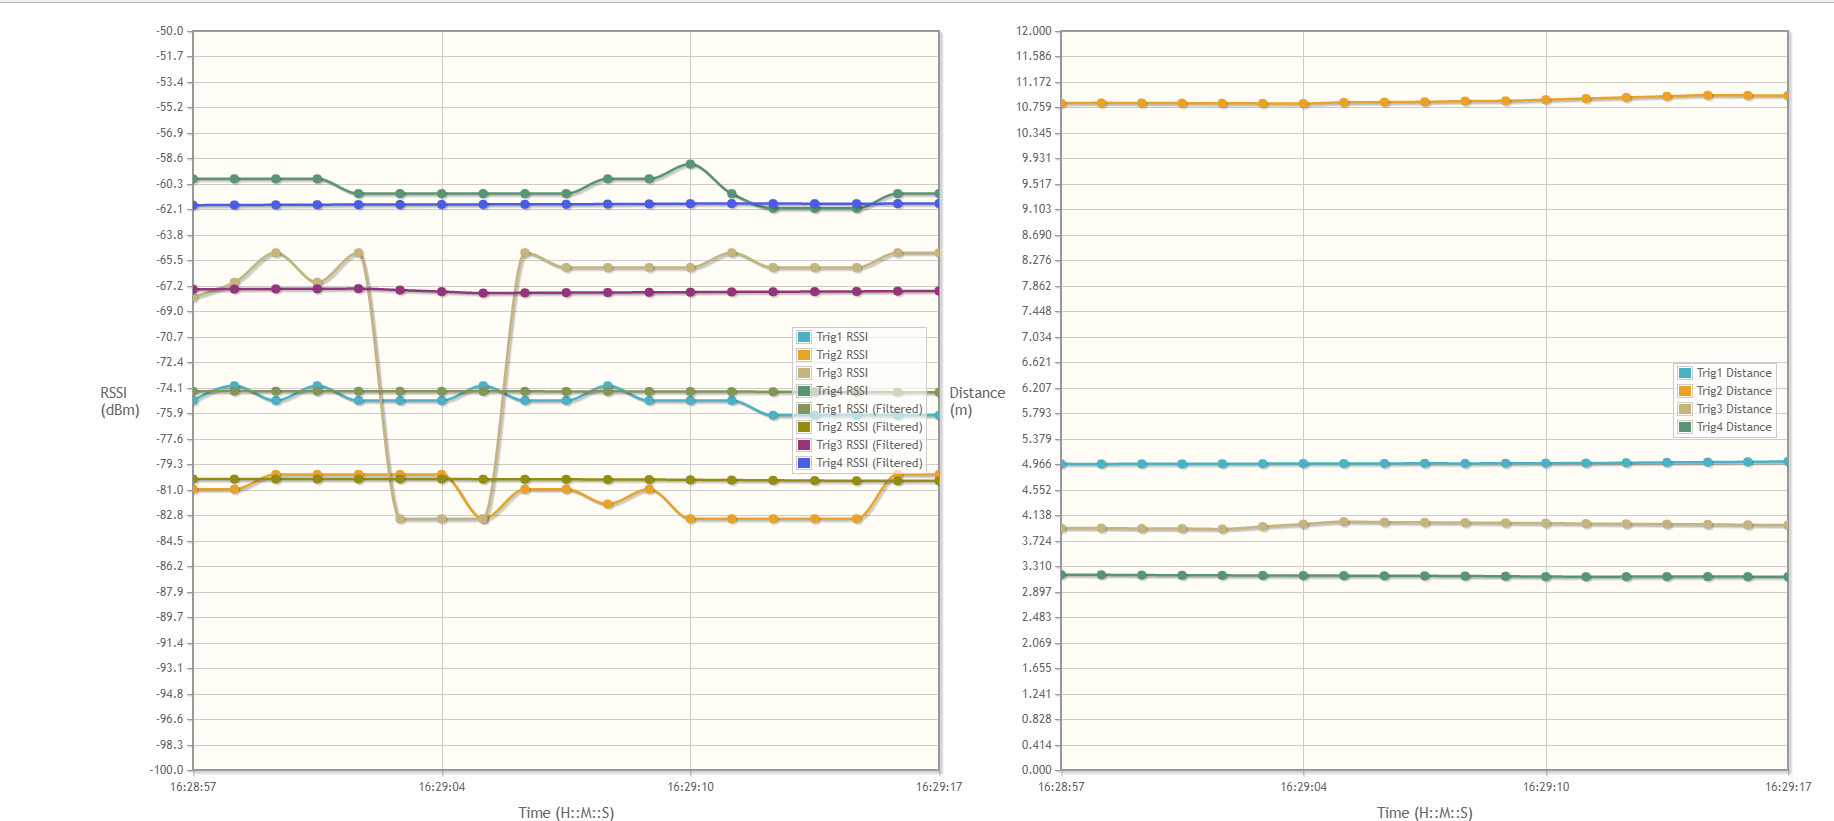
\includegraphics[width=8cm,height=5cm]{2018-05-10-PHOTO-00000079.png}
    \caption{Kalman Results}
    \end{figure}
\subsubsection{LAPACK Results}
As was mentioned previously in the implementation section, 3 methods were utilized for solving the system of equations. DGELS solves an over or underdetermined system using QR or LQ factorization of A. DGESV, solves an over or underdetermined system through partial pivoting and row interchanges to factorize A. The factored form of A, is then used to solve the system of equations. DGETRS simply solves the system of equations, given the LU factorization of A. Since A is essentially a constant, as the AP locations in a facility do not change,the LU factorization of A can be  computed a single time thus enabling DGETRS to be employed to solve the system of equations. This, in theory, should be far less computationally expensive. In order to evaluate the relative "costs" of each of these methods, the time taken for each of these methods to solve the system was measured. The results can be seen below:\newline
18000 ns DGELS\newline
10000 ns DGESV\newline
6000 ns DGETRS\newline
As one can see, DGETRS is almost three times cheaper than DGELS and as such, if this system were to be synthesized for hardware or low-level system software it would be of benefit to utilize DGETRS instead of DGELS or DGESV wherever possible. However, it is worth noting that at least one call to DGESV will be required to derive the factorized A component.
\subsubsection{Location Results}
The system was tested in a relatively "noisy" engineering environment with electromagnetic interference and large multipath losses. The third floor of the SDSU Engineering Building was the chosen environment. The test platform was found to have a scan refresh rate of around 2 Hz. There was also a settle time of ~ 10 seconds for the Kalman Filter. However, an error of approximately 3m was evident in areas of good wireless coverage (Less than 10m to each AP) such as in Figure 7.
\begin{figure}[H]
    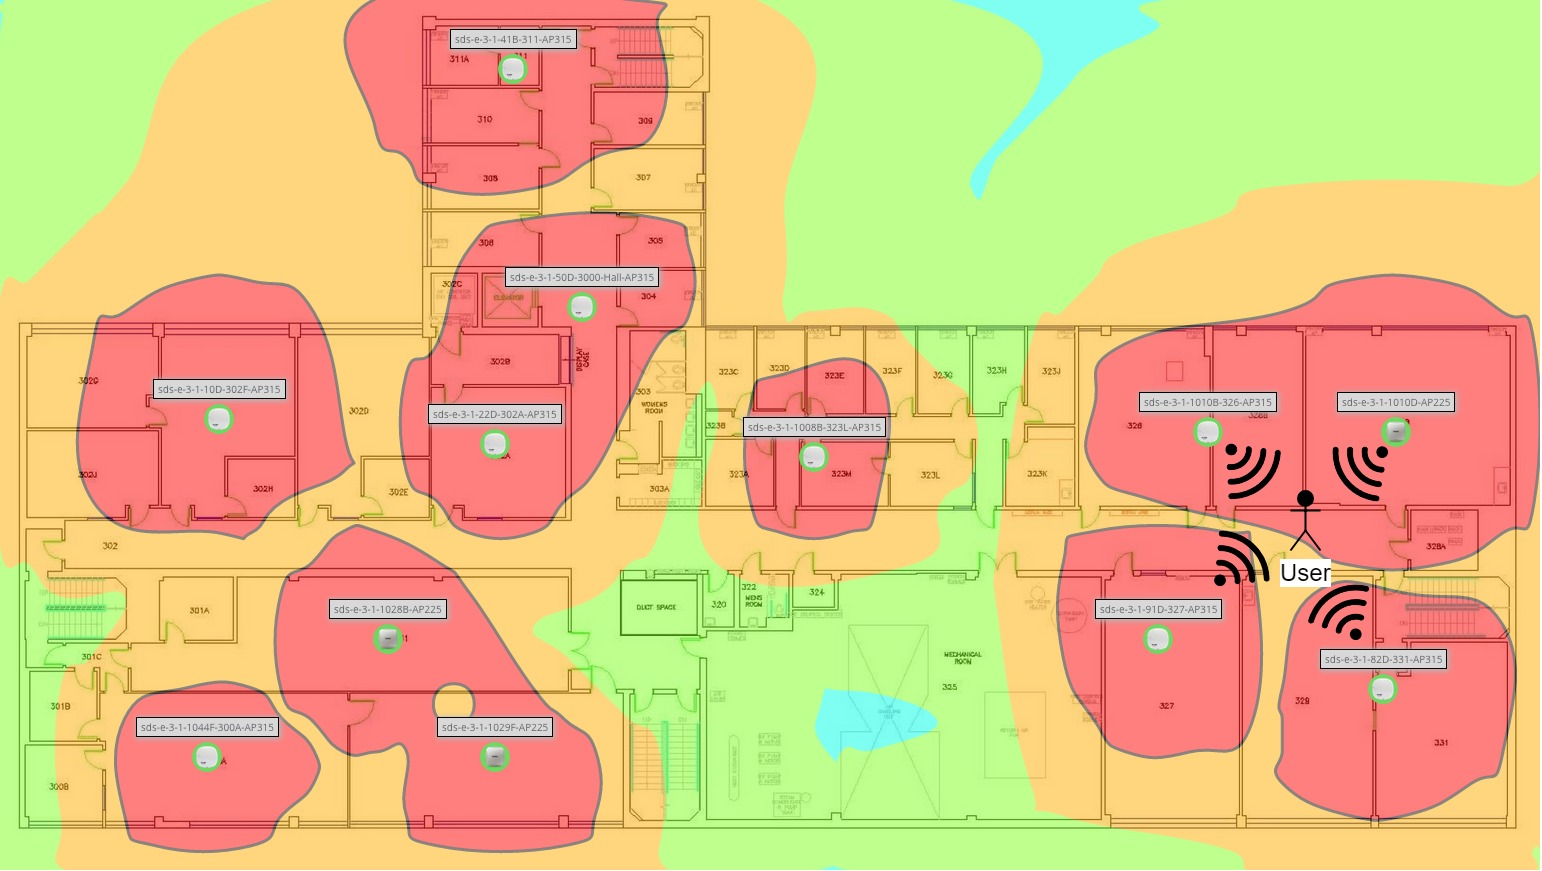
\includegraphics[width=9.0cm,height=6cm]{Geolocation_1.jpeg}
    \caption{Example of Good Coverage}
    \end{figure}


In areas of poorer coverage, an error of approximately 10m was present. Poorer coverage is designated as any situation where there it is more than 15m to 2 or more APs or in areas of high interference and/or path loss. (See Figure 8)
\begin{figure}[H]
    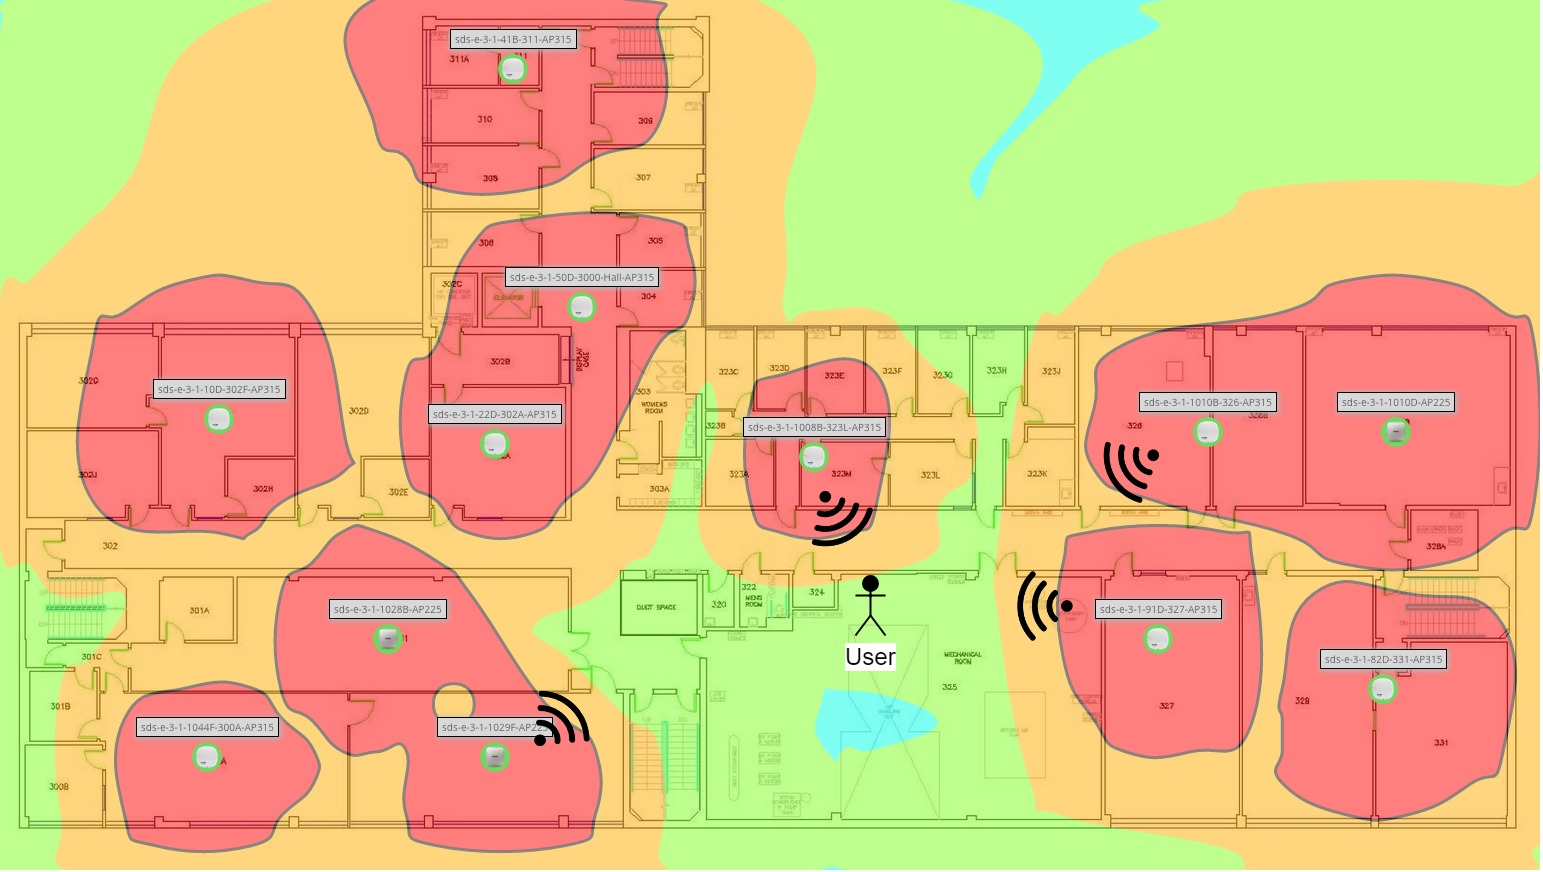
\includegraphics[width=9.0cm,height=6cm]{Geolocation_2.jpeg}
    \caption{Example of Poor Coverage}
    \end{figure}

However, there is a key limitation of the system and that is its inability to differentiate between signal attenuation due to distance and signal attenuation due to obstacle-induced path loss. This means that the system may derive the location of the individual to be in the left corner of the map, outside the building boundaries instead of their actual location as shown in Figure 9.
\begin{figure}[H]
    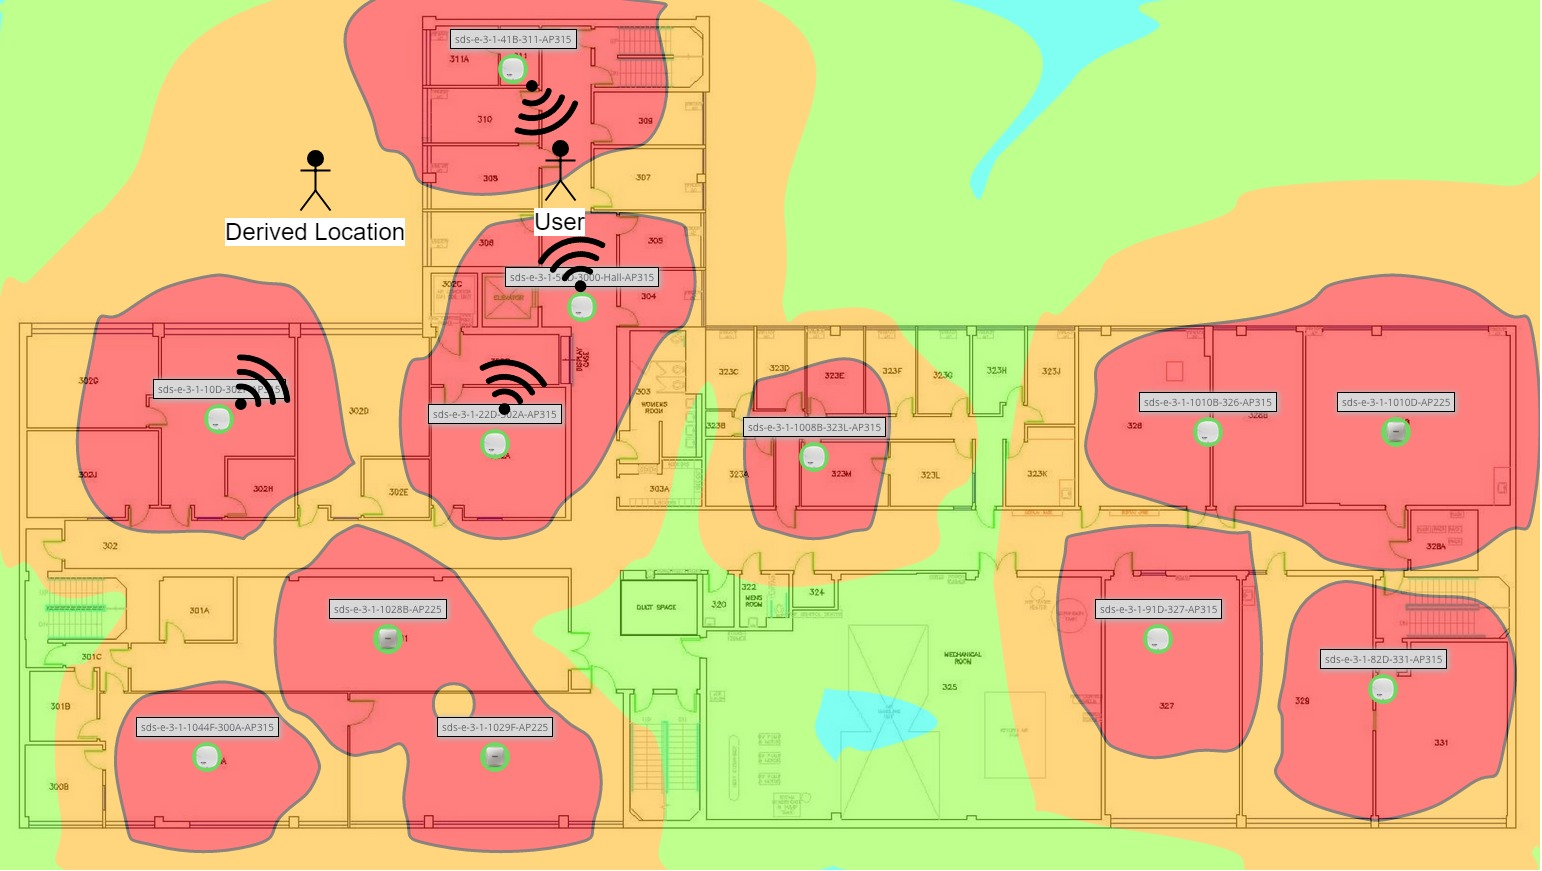
\includegraphics[width=9.0cm,height=6cm]{Geolocation_3.jpeg}
    \caption{Example of incorrect location deduction}
    \end{figure}

\section{Further Work}
As one can see, the developed system is fully capable of deriving the location of a user, assuming that 4 or more known access points are within range. However, a number of areas are avenues for future work. The employment of machine learning technologies could help improve the accuracy of the derived location, for example. One use of this technology could include measuring the wireless signal strengths at several "known locations" within a facility. This information could then be used to generate a set of decision trees which could be employed by the system to enable it to more accurately derive the location. Furthermore, the mobile application and Web services developed in this paper are a proof of concept that will need to be expanded to support multiple clients. As was previously mentioned, the advantage of this software framework is that it can be easily compiled and run on several platforms by simply developing platform specific scan module implementations. Future work will include the implementation of several platform specific modules for iOS, Android, and Windows.

\section{Conclusion}

This paper has successfully out laid the development of a multiplatform, indoor, Geolocation framework compatible with 802.11 protocol. The system is capable of deriving location to within an accuracy 3m and is also portable across multiple platforms. The complete solution provides an end to end framework for monitoring individuals from a mobile device and the software framework provides huge scope for expansion and future feature implementation. The system employs modern C++11 and OOP design principles and as a result is portable, expandable, thread safe and memory safe. The performance of the system has been profiled and a number of areas for further development have been outlined. As such this project has successfully met the goals of developing an affordable, Open Source Indoor Geolocation framework for tracking the location and movements of individuals. It is hoped that this technology will be employed and used in the future to help reduce the time it takes for individuals in need of care to be located, thus saving lives.
\printbibliography
\end{document}